\documentclass{paper}
\usepackage{mathrsfs,amsmath, wasysym, geometry, pstricks, graphicx, type1cm, lettrine, float, fancyhdr}
\usepackage[super]{nth}
\geometry{a4paper}
\usepackage{algorithm}
\usepackage{algpseudocode}
\usepackage{graphicx}
\usepackage{microtype}
\usepackage{pdfpages}
\PassOptionsToPackage{hyphens}{url}\usepackage{hyperref}\usepackage{hyperref}

\newcommand{\HRule}{\rule{\linewidth}{0.5mm}}
\usepackage{listings}
\definecolor{mygreen}{rgb}{0,0.6,0}
\definecolor{mygray}{rgb}{0.8,0.8,0.8}
\definecolor{mymauve}{rgb}{0.58,0,0.82}

\pagestyle{fancy}
\lhead{Storm \emph{Proposal}}
\lfoot{QUT EESS}

\begin{document}
\newpage
\begin{titlepage}
\begin{center}

\textsc{\LARGE ENB440 RF Techniques and Modern Applications}\\[0.75cm]

\begin{figure}[H]
\centering

\includegraphics[width=0.2\textwidth]{IMG/QUT} \\[0.75cm]
\end{figure}

\textsc{\Large ENB440 - Filter Design}\\[0.5cm]

% Title
\HRule \\[0.4cm]
{ \huge \bfseries Design Milestone 1 \\[0.4cm] }

\HRule \\[1.5cm]



\begin{minipage}{0.4\textwidth}
\begin{flushleft} \large
Grant \textsc{Kennedy} \\
\emph{n8566712}\\
\end{flushleft}
\end{minipage}
\begin{minipage}{0.4\textwidth}
\begin{flushright} \large
Blake \textsc{Fuller} \\
\emph{n8598819}\\
\end{flushright}
\end{minipage}

\vfill

% Bottom of the page
{\large \today}
\end{center}
\end{titlepage}

\section*{Executive Summary}
In this report a 70$\Omega$ microstrip is characterised through mathematic calculation, then designed and modeled within the CST Design Suite software environment.\\

Transmission and reflection characteristics are first calculated in section ~\ref{SECTION} in terms of ABCD parameters, from which the geometry of the system is calculated. The microstrip geometries are then independently found by using TX-Line software in section ~\ref{sec:tx-line}.\\

CST modeling methods and S parameters are evaluated in section ~\ref{sec:CST}. Passband, return loss and transmission are discussed in terms of the microstrip S parameters.\\

\textbf{talk about conclusion}





\newpage
\tableofcontents

\newpage
\section{Scope}


\newpage
\section{Line Impedance Calculations}
\subsection{Hand Calculations}
`

\subsection{Computer Generated Results}
\label{sec:tx-line}
The National Instruments (NI) program TX-Line was used to generate an approximation of the microstrip geometry. The given laminate, impedance, frequency and electrical length information were input and the program output the microstrip width and length. \\

These values can be seen in the TX-Line GUI screenshop in figure ~\ref{fig:txline}  

\begin{figure}[H]
	\centering
	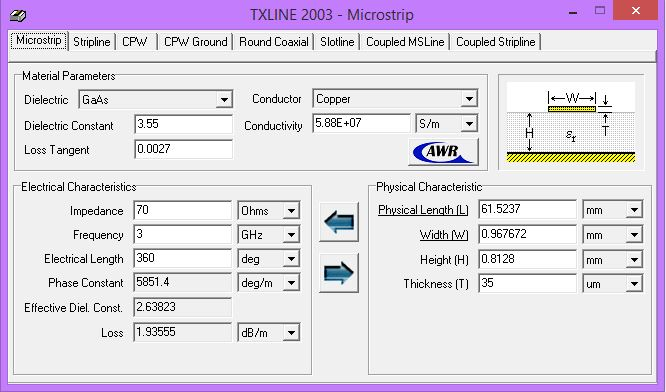
\includegraphics[scale=0.6]{IMG/txline}
	\caption{Screenshot of TX-Line program.}
	\label{fig:txline}
\end{figure}

The following data was found from the results:

\begin{center}
	\begin{tabular}{c|c}
		\hline
		Characteristic & Result\\\hline\hline
		Phase Constant & 0.102126 rad/mm\\\hline
		Physical Length & 61.5237 mm\\	\hline
		Width & 0.967672 mm\\\hline
		Eff. Diel. Const. & 2.63823\\\hline
	\end{tabular}
\end{center}

\newpage
\section{Modeling}
\label{sec:CST}
The microstrip was modeled in CST, with a frequency range of 2GHz to 4GHz and port information defined at 3GHz. The computer generated results found from TX-Line were initially used and resulted in the model that can be seen below in figure ~\ref{fig:stripline1}.\\

\begin{figure}[H]
	\centering
	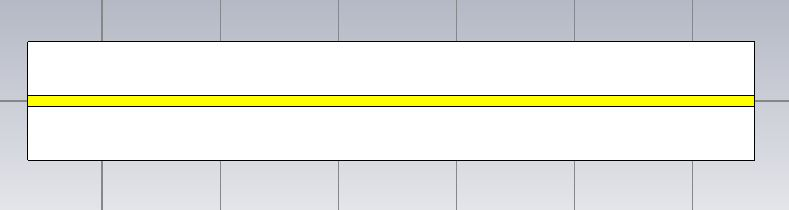
\includegraphics[scale=0.5]{IMG/CSTStripline}
	\caption{CST Microstrip model.}
	\label{fig:stripline1}
\end{figure}

The reflection (S$_{11}$ and S$_{22}$) and transmission S parameters (S$_{21}$ and S$_{12}$) were then found after simulation. These can be seen below in figure ~\ref{fig:s11_s22_s21_s12}.

\begin{figure}[H]
	\centering
	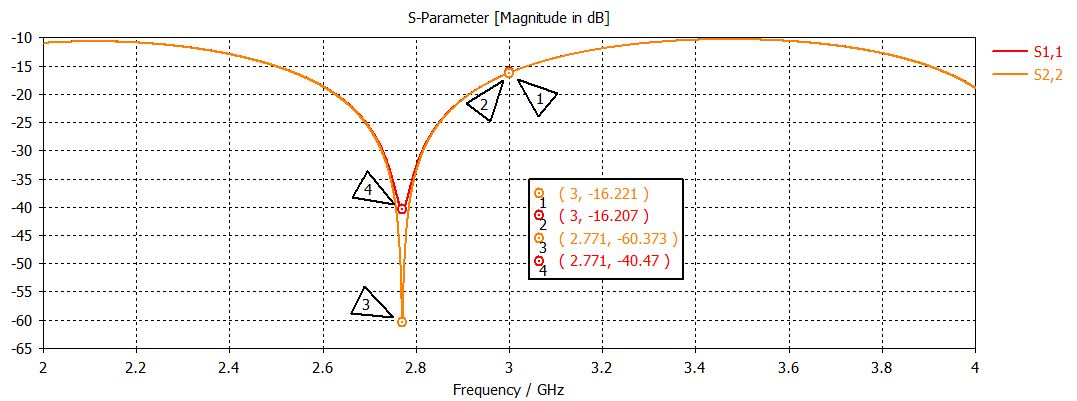
\includegraphics[scale=0.4]{IMG/S11_and_S22}
	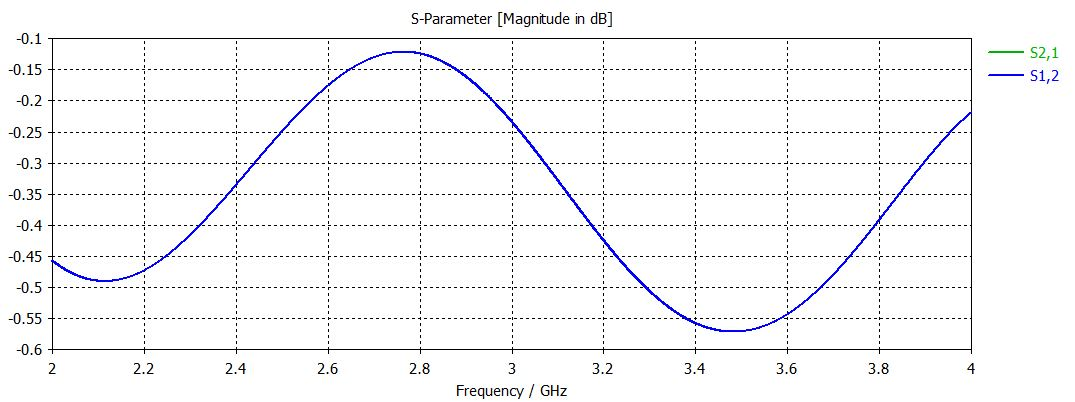
\includegraphics[scale=0.4]{IMG/S21_and_S12}
	\caption{Top: S$_{11}$ and S$_{22}$ parameters - magnitude. Bottom: S$_{21}$ and S$_{12}$ parameters - magnitude.}
	\label{fig:s11_s22_s21_s12}
\end{figure}

It can be seen that the loss of the microstrip along the transmission S parameter $S_{21}$ is 0.239dB. This value is expected - the loss in the copper and dielectric would result in a low loss, especially given the loss tangent of RO4003C being as low as 0.0027.\\

The passband of the system is seen to peak at 2.771GHz with very little loss (passband at -60dB S$_{11}$ and -40dB S$_{22}$). At the specified transmission frequency of 3GHz the reflection of the microstrip is -16dB, causing return losses. The cause of this is the mismatch between the 50$\Omega$ source port and the 70$\Omega$ microstrip.\\

The phase of all S parameters can be seen below in figure ~\ref{fig:s11_s22_s21_s12_phase}.\\

\begin{figure}[H]
	\centering
	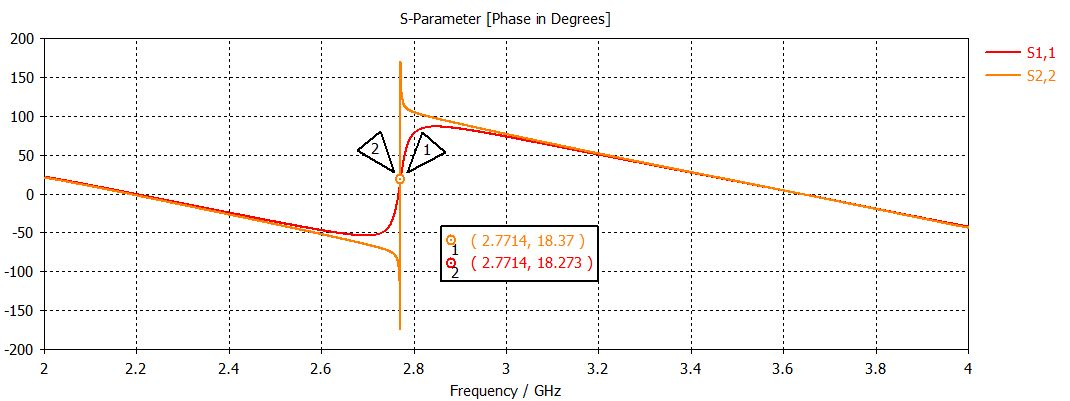
\includegraphics[scale=0.4]{IMG/S11_and_S22_phase}
	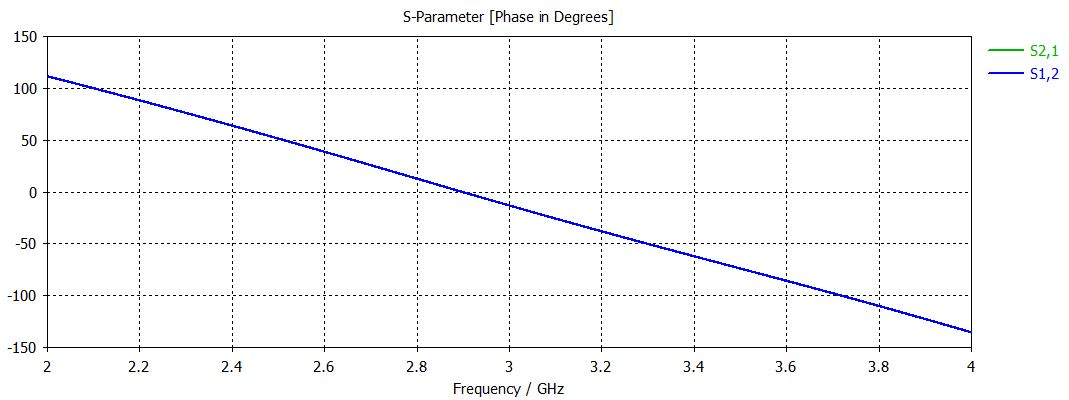
\includegraphics[scale=0.4]{IMG/S21_and_S12_phase}
	\caption{Top: S$_{11}$ and S$_{22}$ parameters - phase. Bottom: S$_{21}$ and S$_{12}$ parameters - phase.}
	\label{fig:s11_s22_s21_s12_phase}
\end{figure}


All S parameter phase plots are linear, as expected. \\

The S$_{11}$ and S$_{22}$ plots have an abnormality at 2.7714GHz, which is caused by the passband peak.\\

\subsection{CST Optimiser}
The CST optimisation software 





\end{document}